\documentclass[10pt]{article}

\usepackage[a4paper,top=1in,bottom=1in,left=1in,right=1in]{geometry}
\usepackage{amsmath, amssymb}
\usepackage{graphicx}
\usepackage{float}
\usepackage{titlesec}
\usepackage{enumitem}
\usepackage{setspace}
\usepackage{parskip}
\usepackage{tikz}
\usetikzlibrary{arrows.meta, positioning, fit, backgrounds, calc, shapes.geometric}
\usepackage{pgfplots}
\pgfplotsset{compat=1.18}
\usepackage[numbers,sort&compress]{natbib}
\usepackage{hyperref}
\usepackage{xurl}
\usepackage[colorinlistoftodos, textsize=footnotesize]{todonotes}
\usepackage{marginnote}
\usepackage{pdfcomment}

% \leftnote[Subject]{word to highlight}{popup text}
% Highlights a word in yellow; hover to reveal the popup note.
% Usage: \leftnote[Definition]{SLAs}{SLA = Service Level Agreement...}
\newcommand{\leftnote}[3][Note]{%
  \pdfmarkupcomment[color={1 0.95 0.4},markup=Highlight,author={#1},
    hoffset=-400pt, voffset=50pt]{#2}{#3}%
}
\setstretch{1.0}
\setlength{\parindent}{0pt}
\setlist[itemize]{leftmargin=1.2em}

\titleformat{\section}{\large\bfseries}{\thesection.}{0.6em}{}
\titleformat{\subsection}{\normalsize\bfseries}{\thesubsection}{0.6em}{}

\title{\textbf{Simple and Scalable Probabilistic Correction\\
for Space Domain Awareness}}
\author{Anonymous}
\date{} 

\begin{document}
\maketitle
%\listoftodos  % remove this line before final submission

\section*{Executive Summary}

Space Domain Awareness (SDA) is a foundational capability for ensuring the safety, resilience, and operational superiority of United States (U.S.) space assets. The rapid growth of satellites and orbital debris is significantly increasing the frequency of close approaches between space objects, making reliable collision-risk assessment a critical operational challenge for civil and defense space agencies.

Conjunction assessment (CA) is the operational process used by the U.S. Space Force to detect potential collisions and estimate the probability of collision between space objects. Operational units such as the 18th and 19th Space Defense Squadrons perform catalog-wide conjunction screenings multiple times per day to protect national space assets and maintain custody of the space environment. As the orbital environment becomes increasingly congested, these systems must scale to analyze tens of thousands of objects while maintaining reliable risk estimation and manageable operator workload.

A major limitation in current conjunction assessment pipelines is the difficulty of accurately propagating uncertainty during multi-day orbit forecasts. Small modeling errors accumulate over time, leading to miscalibrated covariance estimates. These inaccuracies propagate directly into probability-of-collision (Pc) calculations, producing unstable risk estimates, inflated false alerts, and degraded maneuver decision support for operators.

This proposal introduces a \textit{Continuous-Time Probabilistic Corrector (CTPC)}, a transition-compatible module designed to augment existing orbital propagators with a statistically calibrated uncertainty model. Rather than replacing current operational SDA systems, CTPC integrates as a lightweight probabilistic correction layer between deterministic propagation and downstream Pc computation. This architecture preserves compatibility with existing SDA pipelines while improving long-horizon forecasts accuray and uncertainty calibration.

By improving covariance realism and stabilizing collision-risk estimation, the proposed capability aims to reduce false alert volumes, improve operator decision confidence, and enable scalable safety monitoring for the rapidly growing space catalog. These advances directly support national priorities in space traffic management, orbital debris mitigation, and resilient space operations.

\section{Problem Context}

SDA relies on continuous monitoring of the orbital environment to maintain custody of resident space objects and assess potential collision risks. Within this architecture, CA plays a central operational role by identifying close approaches between objects and estimating the probability of collision to support maneuver decision-making.

Operational CA pipelines must screen tens of thousands of cataloged space objects multiple times per day. For each screening cycle, candidate close approaches are identified, propagated to the predicted time of closest approach (TCA), and evaluated using Pc algorithms that depend on the relative state uncertainty of the objects involved. These computations must be repeated continuously as new observations are incorporated and orbital states are updated.

Deterministic orbital propagation between observation updates is typically performed using high-fidelity tools such as the General Mission Analysis Tool (GMAT), which accurately advances nominal orbital states under known force models. However, during extended open-loop propagation, systematic modeling errors accumulate due to environmental uncertainty, force model mismatch, and unmodeled impulsive events.

A critical challenge arises in the propagation of uncertainty during these forecast horizons. In operational workflows, covariance evolution is commonly approximated using linearized propagation or heuristic process-noise tuning for computational efficiency. While these approximations are tractable at catalog scale, they can produce systematic covariance miscalibration over longer propagation intervals.

Because probability-of-collision calculations depend directly on the relative covariance of the objects at TCA, inaccuracies in uncertainty propagation propagate directly into collision-risk estimates. Underestimated covariance can produce overconfident predictions and degraded maneuver detection sensitivity, while overestimated covariance inflates alert volumes and increases analyst workload. Downstream Pc computation, such as the Hall 3D implementation within the CARA SDK~\cite{hall2021_3dnc, hall2023_pcmultistep, cara_sdk_multistep}, is therefore highly sensitive to upstream covariance quality. In practice, miscalibrated uncertainty can lead to unstable Pc estimates across successive updates and complicate alert prioritization.

The operational importance of improving uncertainty calibration is reinforced by several mission-level drivers:

\begin{itemize}
    \item \textbf{National policy priority:} Recent U.S. policy direction emphasizes space traffic management and orbital debris mitigation, increasing the need for reliable collision-risk estimation and maneuver support~\cite{whitehouse_space_superiority_2025}.
    
    \item \textbf{Operational tempo:} Conjunction screening is performed multiple times daily across the full satellite catalog~\cite{nasa_cara, nasa_bestpractices}, meaning that even small covariance errors can scale into substantial false alerting and analyst workload at operational tempo.
    
    \item \textbf{Technology shortfalls:} NASA assessments identify mitigation of new orbital debris generation as a critical capability gap, for which improved conjunction assessment is a key enabling capability~\cite{nasa_civil_space_shortfall_2024}.
    
    \item \textbf{SDA mission dependency:} Recent analyses highlight conjunction assessment as a core SDA function and identify uncertainty quantification as a key enabler for trustworthy Artificial Intelligence \& Machine Learning (AI/ML) integration into operational SDA pipelines~\cite{rand_rra2318_1, rand_rra2318_2}.
    
    \item \textbf{Global congestion trends:} European Space Agency (ESA) reporting indicates sustained growth in debris populations and collision-relevant objects, increasing the frequency of close approaches and the operational value of scalable collision risk assessment methods~\cite{esa_space_environment_report_2025}.
    
    \item \textbf{Observation constraints:} Space Surveillance Network (SSN) sensors serve multiple mission priorities, limiting on-demand tracking availability and producing uneven observation cadence across objects~\cite{nasa_bestpractices, spacetrack_handbook}. These constraints further increase the importance of robust long-horizon uncertainty forecasting.
\end{itemize}

Together, these operational and policy drivers establish that improving long-horizon uncertainty calibration is not merely a research objective but a practical requirement for scalable, reliable conjunction assessment within modern SDA systems.

\section{Problem Statement}\label{sec:prob_statement}

Current CA pipelines exhibit several operational limitations that degrade the reliability and scalability of collision-risk assessment as the space object catalog continues to expand.

\begin{itemize}

\item \textbf{Calibration gap:} Over multi-day propagation horizons, the statistical consistency of propagated uncertainty deteriorates. In practice, the squared Mahalanobis distance between predicted states and subsequent orbit updates deviates from its expected chi-square ($\chi^2$) distribution, indicating covariance miscalibration. This produces several well-documented operational failure modes reported in NASA best-practices literature~\cite{nasa_bestpractices, hejduk2015}, including:
\begin{itemize}
    \item \textit{Probability dilution}, where inflated covariance artificially depresses computed $P_c$;
    \item \textit{$P_c$ bias}, where estimated collision risk systematically deviates from the true likelihood of collision;
    \item \textit{$P_c$ thrash}, where successive conjunction data message (CDM) updates produce large fluctuations in estimated $P_c$ for the same event.
\end{itemize}

\item \textbf{Alert burden gap:} Miscalibrated covariance increases the number of false-positive conjunction alerts, forcing operators to investigate events that do not represent credible collision risks. As screening is performed repeatedly across the full satellite catalog, these false alerts accumulate and increase analyst workload.

\item \textbf{Runtime gap:} High-fidelity uncertainty characterization using Monte Carlo (MC) propagation is computationally expensive. Operational MC analysis requires propagating thousands of sampled trajectories for each conjunction event. At catalog scale, with multiple daily screenings across tens of thousands of objects, brute-force MC propagation becomes impractical for routine use.

\end{itemize}

The core challenge is therefore not deterministic orbit propagation accuracy alone, but the reliable calibration of uncertainty over multi-day horizons at catalog scale. This proposal addresses this limitation through the CTPC corrector, which augments physics-based propagators (e.g., GMAT) with a learned probabilistic correction model. The approach preserves compatibility with existing propagation and $P_c$ computation pipelines while improving uncertainty calibration and reducing downstream alert burden.

\section{Proposed Solution Concept}

%As the space environment becomes increasingly congested, operational safety tools must scale to catalog-level analysis involving tens of thousands of objects while remaining trustworthy in safety-critical decision pipelines. In such environments, reliability is closely tied to algorithmic transparency and verifiability. 
Highly complicated ML architectures are difficult to interpret, validate, and certify for operational use. Our design philosophy therefore prioritizes \textit{interpretable simplicity}, i.e., safety-critical space analytics should rely on simple ML architectures that remain interpretable, mathematically grounded, and operationally verifiable. Rather than replacing physics-based systems with blackbox models, we introduce lightweight learning components that augment existing analytical frameworks while preserving their interpretability and safety properties. This approach enables scalable deployment, facilitates verification of algorithmic behavior, and supports operator trust in automated risk assessments.

To address the calibration gap identified in \textbf{Section}~\ref{sec:prob_statement}, we introduce a CTPC corrector that augments rather than replaces existing SDA infrastructure. CTPC learns the systematic forecast error dynamics of deterministic propagators (e.g., GMAT) and uses this knowledge to produce calibrated uncertainty for the forecasts before collision risk evaluation.

The CTPC correction layer wraps around any deterministic propagator and is inserted between deterministic propagation and downstream Pc evaluation. As illustrated in Figure~\ref{fig:ctpc-placement}, this integration acts as a non-disruptive augmentation to existing SDA pipelines.

\begin{figure}[htbp]
\centering
\resizebox{\linewidth}{!}{%
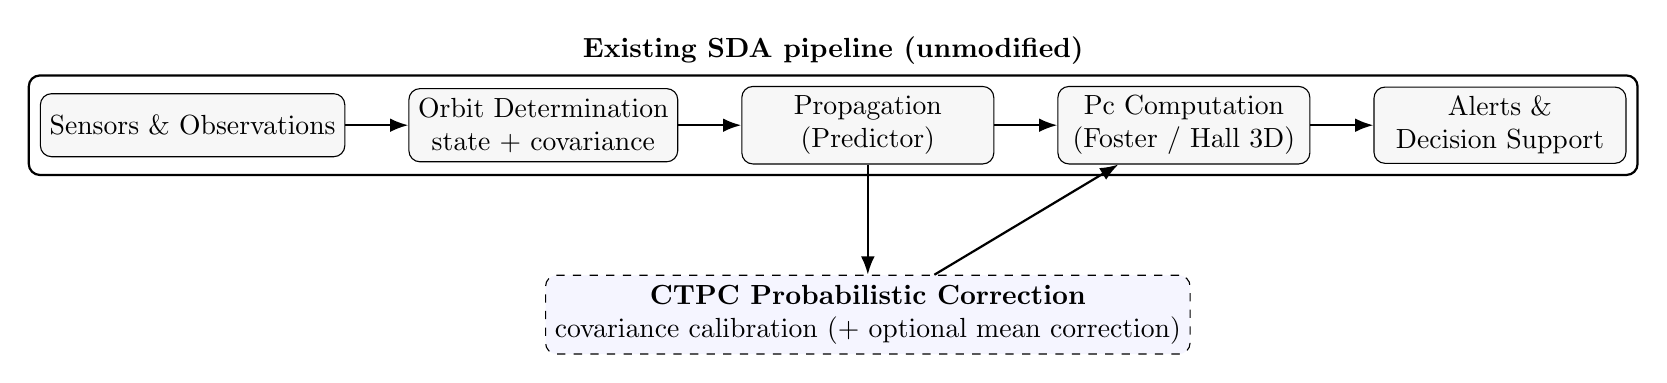
\begin{tikzpicture}[
  node distance=8mm and 8mm,
  box/.style={draw, rounded corners, align=center, minimum width=3.2cm, minimum height=8mm, fill=gray!6},
  cbox/.style={draw, dashed, rounded corners, align=center, minimum width=4.0cm, minimum height=10mm, fill=blue!4},
  arrow/.style={-Latex, thick}
]
\node[box] (s) {Sensors \& Observations};
\node[box, right=of s] (od) {Orbit Determination\\state + covariance};
\node[box, right=of od] (prop) {Propagation\\(Predictor)};
\node[box, right=of prop] (pc) {Pc Computation\\(Foster / Hall 3D)};
\node[box, right=of pc] (ds) {Alerts \&\\Decision Support};
\draw[arrow] (s) -- (od);
\draw[arrow] (od) -- (prop);
\draw[arrow] (prop) -- (pc);
\draw[arrow] (pc) -- (ds);
\node[cbox, below=14mm of prop] (ctpc) {\textbf{CTPC Probabilistic Correction}\\covariance calibration (+ optional mean correction)};
\draw[arrow] (prop) -- (ctpc);
\draw[arrow] (ctpc) -- (pc);
\node[draw, thick, rounded corners, fit=(s)(ds), inner sep=4pt, label=above:{\textbf{Existing SDA pipeline (unmodified)}}] {};
\end{tikzpicture}%
}
\caption{CTPC placement as a non-disruptive add-on between propagation and Pc computation.}
\label{fig:ctpc-placement}
\end{figure}

The correction layer consumes deterministic propagated states together with operational metadata (e.g., observation history) and outputs a calibrated uncertainty for the deterministic forecasts. The deterministic propagator itself remains unchanged. Instead, CTPC models systematic forecast error dynamics learned from historical conjunction data and produces over the entire forecast horizon:

\begin{itemize}
\item Corrected mean forecasts
\item Full positive semi-definite covariance matrix
\item \leftnote[Heavy Tail Behavior]{Calibrated}{See if you can elaborate the extreme error capturing in an elegant way} uncertainty ellipsoids capable of capturing rare deviations. This property of capturing rare deviations helps with maneuver detection using sequential hypothesis testing (\textbf{Section}~\ref{sec:maneuver_detection}).
\end{itemize}

Importantly, this architecture preserves compatibility with existing CA infrastructure. No modification to downstream Pc algorithms, CDM schemas, or operational decision-support tools is required. As a result, CTPC can be deployed as a low-disruption enhancement within current operational SDA pipelines.

Because the correction targets covariance \textit{realism} rather than simple conservatism, it directly mitigates probability dilution and Pc bias. This design claim is evaluated through the \hyperref[itm:pdi]{\textit{probability-dilution incidence rate}}, i.e., the fraction of conjunction updates classified as dilution-like under NASA-consistent definitions.

\textbf{Operational Design Properties}

The CTPC framework is designed to satisfy the key requirements of safety-critical conjunction assessment systems:

\begin{itemize}
\item Continuous-time formulation supporting arbitrary forecast horizons
\item Full covariance ellipsoids capturing correlated uncertainty growth
\item Positive semi-definite covariance guaranteed by construction
\item Robust modeling of rare deviations through heavy-tailed uncertainty ellipsoids
\item Proper scoring-rule training to promote statistical calibration
\item Bounded uncertainty growth under nominal operating conditions
\item Conservative fallback behavior under anomalous regimes
\item Single-pass inference at runtime, enabling millisecond-scale processing per conjunction event at catalog scale
\end{itemize}

\section{Technical Approach}

The technical approach is organized around three primary objectives. \textbf{Section}~\ref{sec:ctpc_correction} presents an overview of the the proposed probabilistic correction mechanism. \textbf{Section}~\ref{sec:maneuver_detection} presents maneuver/anomaly detection using sequential hypothesis testing. \textbf{Section}~\ref{sec:BayesOpt_planning} presents risk-aware maneuver planning based on probabilistic safety constraints. The three components are integrated in architecture and evaluated with objective-specific criteria within a transition pathway towards operational space safety.

\subsection{Core CTPC Methodology}\label{sec:ctpc_correction}

\begin{figure}[htbp]
    \centering
    \includegraphics[width=0.75\linewidth]{figures/methodology.pdf}
    \caption{High-level CTPC Probabilistic Correction: forecasts of Primary \& Secondary objects are generated by the Predictor, corrected by the CTPC while generating calibrated error ellipsoids, and passed to the Pc computation and maneuver-safety optimization framework. The letter $\tau (=10^{-4})$ and BayesOpt. stands for NASA's safety threshold and Bayesian Optimization, respectively. }
    \label{fig:methodology}
\end{figure}

Figure~\ref{fig:methodology} presents an overview of the proposed safe maneuver planning framework. Current observations for both the primary and secondary objects are propagated by the deterministic Predictor (e.g., GMAT) to TCA. The CTPC Corrector then updates each forecated trajectory with a mean correction and calibrated uncertainty ellipsoid. These corrected state/covariance enters the conjunction-risk layer, where probabilistically safe maneuver regions are identified using risk-aware Bayesian Optimization (BO) (\textbf{Section}~\ref{sec:BayesOpt_planning}). This preserves the existing SDA operational pipeline while improving the quality of upstream uncertainty inputs.

Figure~\ref{fig:ctpc-corrector} provides an overview of our proposed CTPC corrector represented as Corrector in Figure~\ref{fig:methodology}. At this level, CTPC is treated as an encoder-decoder architecture wherein the encoder summarizes recent $T_p$ forecast errors into a latent uncertainty state; samples from that state initialize the decoder; and the decoder propagates uncertainty over the open-loop horizon to produce corrected forecasts ($\hat{\mathbf{x}}_{\text{ECI}}^{\text{corr}}$) and their corresponding error ellipsoids. Specifically, the decoder predicts $\mu_{e}(t)$ \& $\Sigma_{e}(t)$, with $\mu_{e}(t)$ used to correct forecasts' error and $\Sigma_{e}(t)$ to produce sharp and calibrated error ellipsoids. This output is a drop-in replacement for the covariance that would otherwise enter the Pc engine. No changes are required downstream: the Hall 3D method, CDM schema, and alert logic are all preserved~\cite{hall2021_3dnc, ccsds_cdm}.

\begin{figure}[H]
    \centering
    \includegraphics[width=\linewidth]{figures/CTPC_Corrector.pdf}
    \caption{CTPC Corrector: an encoder summarizes recent forecast errors into a latent uncertainty state, and a decoder propagates this state to produce corrected
  forecasts and calibrated error ellipsoids for downstream Pc computation.}
    \label{fig:ctpc-corrector}
\end{figure}

\textbf{Key design properties.} The CTPC corrector is trained on nominal historical trajectories using strictly proper scoring-rule objectives~\cite{gneiting2007strictly} to balance sharpness and calibration. The continuous-time formulation supports irregular observation cadence and tracking gaps~\cite{spacetrack_handbook}, and uncertainty is represented as heavy-tailed full covariance for robustness to outliers. 
%Training uses high-accuracy covariance-bearing catalog products~\cite{spacetrack_handbook}; TLE/SGP4-only products are excluded for covariance-critical Pc analysis~\cite{vallado2006}.

\subsection{Maneuver and Anomaly Detection}
\label{sec:maneuver_detection}

This module reuses the calibrated innovation sequence from \textbf{Section}~\ref{sec:ctpc_correction} and frames maneuver detection as a sequential hypothesis test. Let $\nu_k = S_k^{-1/2}(z_k - \hat{z}_k)$ denote the whitened innovation at observation epoch $k$, where $S_k$ is the CTPC-corrected innovation covariance. Under the null hypothesis $H_0$ (nominal, non-maneuvering dynamics), the calibration guarantee of \textbf{Section}~\ref{sec:ctpc_correction} ensures $\nu_k \stackrel{\text{iid}}{\sim} \mathcal{N}(0,I)$, so the scalar test statistic $d_k^2 = \nu_k^\top \nu_k \sim \chi^2(n)$ is fully characterized. A maneuver or unmodeled impulsive event violates $H_0$ by inducing a persistent mean shift $\mu \neq 0$ in the innovation sequence, shifting $d_k^2$ toward a non-central $\chi^2$ distribution under the alternative $H_1$. 

Detection is implemented via a sliding-window Generalized Likelihood Ratio Test (GLRT). Let $\bar{\nu}_k = \frac{1}{W}\sum_{j=k-W+1}^{k}\nu_j$ denote the windowed sample mean. The GLRT statistic is
\[
\Lambda_k = \frac{W}{2}\left\|\bar{\nu}_k\right\|^2,
\]
where $\hat{\mu} = \bar{\nu}_k$ is the MLE of the shift under $H_1$. A detection is declared when $\Lambda_k > \gamma$, with threshold $\gamma$ set via the Neyman--Pearson criterion at a target false-alarm rate $\alpha$ (e.g., one false declaration per 30 days of catalog screening). Under $H_0$, $2\Lambda_k \sim \chi^2(n)$, so $\gamma$ is obtained directly from the $\chi^2$ quantile without Monte Carlo calibration. A CUSUM extension accumulates evidence across epochs to improve sensitivity to small or gradual anomalies, with analytically tractable average run-length properties under $H_0$.

A key operational property is that the test is \emph{covariance-coherent}: the Neyman--Pearson threshold guarantee holds only when $S_k$ is correctly calibrated. If covariance is mis-specified, the $\chi^2$ reference distribution becomes distorted---inflating false alarms during overestimation and suppressing detection during underestimation, the dominant failure modes documented in NASA best-practices literature~\cite{nasa_bestpractices, hejduk2015}. CTPC calibration from \textbf{Section}~\ref{sec:ctpc_correction}  is therefore a prerequisite for principled threshold control, tying Objectives~\hyperref[sec:obj1]{1} and~\hyperref[sec:obj2]{2} together by design.

Maneuver-detection performance is evaluated on historical conjunction events with known maneuver epochs using the metrics defined in \hyperref[sec:obj2]{Objective 2}.

\subsection{Risk-Aware Maneuver Planning}\label{sec:BayesOpt_planning}

Building on the CTPC correction framework, maneuver planning is formulated as a constrained optimization over maneuver parameters $\theta \in \mathbb{R}^d$, %(e.g., $\Delta v$ components and burn epoch):
\[
\min_{\theta}\; \Delta v(\theta)
\quad \text{subject to} \quad
\text{Pc}(\theta) \leq 10^{-4},
\]
where $\text{Pc}(\theta)$ is evaluated at TCA and $10^{-4}$ is NASA's operational threshold for elevated conjunction risk~\cite{nasa_bestpractices, hall2023_pcmultistep}. Rather than sampling a single terminal point from the search hypercube $\Theta \subset \mathbb{R}^d$, each BO iteration samples a terminal Gaussian ellipsoid (mean plus covariance) that defines a candidate terminal density at $t+T_f$. The initial condition is likewise treated as a density using the CTPC-corrected state uncertainty at current epoch $t$. The maneuver energy/fuel cost $\Delta v(\theta)$ is then evaluated by solving the resulting density-to-density transfer with the physics-based optimal-transport algorithm of~\cite{nodozi2023physics}. For conjunction risk evaluation, the maneuvered primary-object terminal density is combined with the propagated secondary-object density to compute $\text{Pc}(\theta)$ at TCA. The two GP surrogates are updated after each evaluation, and the acquisition progressively concentrates on terminal densities in the safe zone (with smaller Pc) while avoiding fuel-expensive regions (see Figure~\ref{fig:safe-zone}).

\begin{figure}[H]
    \centering
    
\includegraphics[width=0.74\linewidth]{figures/safe_zone_viz.pdf}
    \caption{Risk-aware maneuver planning framework: BO samples terminal Gaussian ellipsoids in $\Theta$ at TCA, maneuver cost is computed via density-to-density optimal transport~\cite{nodozi2023physics}, and collision risk $\text{Pc}(\theta)$ is evaluated between the maneuvered primary object's density and propagated secondary object's density.}
    \label{fig:safe-zone}
\end{figure}

\textbf{Risk-Aware Constrained Bayesian Optimization.} Both the fuel cost and the safety constraint are optimized simultaneously within a single BO loop. Two independent GP surrogates are maintained:
\begin{itemize}
    \item $\mathcal{GP}_{\Delta v}$: surrogate for the fuel cost $\Delta v(\theta)$,
    \item $\mathcal{GP}_{\text{Pc}}$: surrogate for the collision probability $\text{Pc}(\theta)$.
\end{itemize}
Standard constrained BO uses a binary feasibility probability $\Pr[\text{Pc}(\theta) \leq 10^{-4}]$, which collapses the full GP posterior to a point estimate and treats all infeasible Pc values equivalently. This is insufficient for safety-critical planning: in unexplored regions of the maneuver space, the GP posterior over Pc$(\theta)$ is wide, meaning the surrogate's nominal Pc estimate carries high uncertainty. Accepting a maneuver solely because its \emph{expected} Pc is below threshold can violate the safety constraint in the true system.

The proposed acquisition instead enforces a risk-aware feasibility condition using the Conditional Value-at-Risk (CVaR) of the GP posterior. At confidence level $\alpha$ (e.g., $\alpha = 0.95$), $\text{CVaR}_\alpha[\text{Pc}(\theta)]$ is the expected Pc in the worst $\alpha$-fraction of outcomes under the posterior predictive distribution of $\mathcal{GP}_{\text{Pc}}$. The risk-aware acquisition function is:
\[
\alpha_{\text{RA}}(\theta) = \underbrace{\mathbb{E}_{\mathcal{GP}_{\Delta v}}\!\left[\max\!\left(\Delta v^* - \Delta v(\theta),\,0\right)\right]}_{\text{expected improvement on }\Delta v} \;\times\; \underbrace{\Pr_{\mathcal{GP}_{\text{Pc}}}\!\left[\,\text{CVaR}_\alpha\!\left[\text{Pc}(\theta)\right] \leq 10^{-4}\right]}_{\text{risk-aware feasibility weight}},
\]
where $\Delta v^*$ is the best feasible cost observed so far. This formulation has two key properties. First, in \emph{unexplored} regions the GP posterior over Pc is wide, yielding high CVaR and near-zero feasibility weight, the acquisition function automatically avoids committing to nominally safe but uncertain maneuvers. Second, in \emph{well-characterized} low-Pc regions the posterior is tight, CVaR collapses toward the mean, and the acquisition concentrates on minimizing fuel cost. The risk-aversion level $\alpha$ is an interpretable operational parameter: $\alpha = 0.95$ requires that the 95th-percentile Pc outcome remain below $10^{-4}$, providing a tunable safety margin beyond the nominal constraint.

The planner converges to the constrained optimum in $O(20$--$50)$ Pc evaluations, tractable even with Hall 3D calls~\cite{hall2021_3dnc}, and the CVaR constraint tightens monotonically as the GP posterior concentrates with more data.

A critical dependency on \textbf{Section}~\ref{sec:ctpc_correction} calibration: $\mathcal{GP}_{\text{Pc}}$ is fit to Pc evaluations computed from CTPC-corrected covariance. If covariance is miscalibrated, the fitted Pc surface is wrong, the GP posterior is mis-centered, and the CVaR constraint provides a false safety guarantee regardless of $\alpha$. Calibrated covariance is therefore a hard prerequisite for risk-aware planning, tying Objective~1 directly to Objective~3.

\section{Evaluation and Success Metrics}\label{sec:evaluation}

The metrics are proposed for three objectives to quantify their performances compared to baselines, e.g., monte carlo.

\textbf{Objective 1 — Probabilistic Correction Performance}\phantomsection\label{sec:obj1}

\begin{itemize}

\item \textbf{Forecast Accuracy (MSE):}
Reduction in corrected state forecast error (Predictor-Corrector) relative to the Predictor-only baseline over multi-day open-loop horizons (2--4 days ahead), measured by mean squared error between the true spacecraft position $\mathbf{x}_\mathrm{ECI}(t)$ and the CTPC-corrected Predictor's forecast $\hat{\mathbf{x}}^\mathrm{corr}_\mathrm{ECI}(t)$:
\[
\mathrm{MSE} = \frac{1}{T - T'} \sum_{t=T'+1}^{T} \bigl\|\mathbf{x}_\mathrm{ECI}(t) - \hat{\mathbf{x}}^\mathrm{corr}_\mathrm{ECI}(t)\bigr\|_2^2.
\]
\leftnote[CTPC-Paper]{Preliminary}{Cite CTPC paper for Preliminary results} results on real spacecraft ephemeris data (NASA CDDIS) show up to 64\% MSE reduction over Predictor (GMAT) alone at 4-day horizons across six rolling test windows from year 2017.

\item \textbf{Calibration (Normalized Mahalanobis Distance):}
Statistical consistency of CTPC's predicted uncertainty is assessed using the squared Mahalanobis distance between the true forecast error $\mathbf{e}_\mathrm{ECI}(t)$ and the predicted error distribution:
\[
d^2_t = \bigl(\mathbf{e}_\mathrm{ECI}(t) - \boldsymbol{\mu}_t\bigr)^\top \boldsymbol{\Sigma}_t^{-1} \bigl(\mathbf{e}_\mathrm{ECI}(t) - \boldsymbol{\mu}_t\bigr).
\]
For a well-specified $D$-dimensional Student-$t$ distribution with $\nu > 2$ degrees of freedom, $\mathbb{E}[d^2_t] = \frac{\nu}{\nu-2}D$. We therefore report the normalized distance
\[
\bar{d}^2_t = \frac{d^2_t}{\dfrac{\nu}{\nu-2}\,D},
\]
\leftnote[CTPC-Paper]{for}{Cite CTPC paper for Preliminary results} which a calibrated predictive distribution satisfies $\mathbb{E}[\bar{d}^2_t] = 1$. Values $\bar{d}^2_t \gg 1$ indicate overconfidence (underestimated uncertainty); values $\bar{d}^2_t \ll 1$ indicate over-diffuse uncertainty. Preliminary results show CTPC maintains $\bar{d}^2_t \approx 0.4$--$1.5$ across all horizons, compared to $\bar{d}^2_t \gg 100$ for Latent ODE baselines~\cite{nasa_bestpractices, hejduk2015}.

\item \textbf{Sharpness (Log-Determinant of Predicted Covariance):}
Sharpness quantifies the concentration of predicted uncertainty independently of the ground truth. It is measured by the log-determinant of the aggregated predicted covariance matrix:
\[
-\log\lvert\bar{\boldsymbol{\Sigma}}_t\rvert = -2\sum_{i=1}^{D} \log (L_t)_{ii},
\]
where $L_t$ is the lower-triangular Cholesky factor of $\bar{\boldsymbol{\Sigma}}_t$. Higher values correspond to tighter uncertainty ellipsoids. Sharpness is interpreted jointly with calibration: a model that achieves good calibration alongside high sharpness produces uncertainty estimates that are both statistically correct and operationally useful for Pc thresholding~\cite{nasa_bestpractices}.

\item \textbf{Probability-Dilution Incidence (PDI):}\phantomsection\label{itm:pdi}
Probability dilution is a well-documented failure mode in operational conjunction assessment~\cite{nasa_bestpractices}: as covariance grows between CDM updates, Pc can paradoxically \emph{decrease} even as the physical threat worsens, creating a false impression of improving safety. This occurs when covariance overestimation inflates the uncertainty volume faster than the miss distance separates the objects. A dilution event at update index $k$ is formally identified by
\[
P_c^{(k+1)} < P_c^{(k)}
\quad \text{and} \quad
\mathrm{tr}\!\left(\Sigma^{(k+1)}\right) > \mathrm{tr}\!\left(\Sigma^{(k)}\right),
\]
and the Probability-Dilution Incidence rate is
\[
\mathrm{PDI}=\frac{N_{\text{dilution events}}}{N_{\text{assessed updates}}}.
\label{eq:pdi}
\]
A reduction in PDI relative to the deterministic-only baseline (or Monte Carlo) is a direct, operationally grounded indicator that CTPC is producing more realistic covariance and reducing the risk of misclassifying high-threat conjunctions as low-priority.

\item \textbf{Operational Efficiency:}
At 18~SDS's screening cadence of three catalog-wide passes per day~\cite{nasa_cara, ussf_18sds}, per-conjunction compute cost accumulates rapidly across tens of thousands of objects. CTPC is designed for faster inference that requires very few trajectory samples (on the order of 100s) compared to Monte Carlo methods (on the order of 1000s)~\cite{hall2023_pcmultistep}. Phase~I benchmarks will report mean and tail-latency per conjunction event against both the deterministic-only pipeline and a Monte Carlo reference, with the explicit metric quanitfying that CTPC introduces small latency regression into the operational screening loop.

\item \textbf{Integration Compatibility:}
A core design commitment of this proposal is non-disruption: CTPC augments the existing SDA pipeline without requiring any modification to downstream Pc engines, CDM schema, or alert logic~\cite{hall2021_3dnc, ccsds_cdm}. Successful shadow-mode operation, running alongside the operational pipeline without influencing its outputs, is among the deliverable. This validate-before-deploy approach is consistent with DoD transition best practices.

\end{itemize}



\textbf{Objective 2 — Maneuver / Anomaly Detection}\phantomsection\label{sec:obj2}

\begin{itemize}

\item \textbf{ROC Area Under the Curve (AUC):}
Measures the intrinsic detection capability of the GLRT by summarizing the trade-off between true-positive and false-positive rates over all decision thresholds $\gamma$. The ROC AUC provides a threshold-independent measure of discriminability between the nominal ($H_0$) and maneuvering ($H_1$) regimes.

\item \textbf{Precision--Recall at the Operational False-Alarm Rate:}
Performance is evaluated at the Neyman--Pearson threshold 
\[
\gamma = F^{-1}_{\chi^2(n)}(1-\alpha),
\]
where $\alpha$ corresponds to the operational false-alarm tolerance (e.g., one false declaration per 30 days of catalog screening). Precision and recall are computed on held-out conjunction events with independently verified maneuver epochs. This evaluates whether the theoretically derived $\chi^2(n)$ reference distribution produced by CTPC calibration achieves the intended Type-I error control in practice.

\item \textbf{Time-to-Detection Statistics:}
Detection latency is defined as the epoch difference between the true maneuver onset and the first epoch for which $\Lambda_k > \gamma$. Mean, median, and $90^{\text{th}}$-percentile latency are reported. This metric captures the responsiveness of the detection system, complementing accuracy metrics. The CUSUM extension is evaluated separately for its sensitivity to small or gradual anomalies where the GLRT window may require several epochs to accumulate evidence.

\item \textbf{Covariance-Coherence Validation:}
During nominal (non-maneuvering) periods, the empirical distribution of the test statistic $2\Lambda_k$ is compared against the theoretical $\chi^2(n)$ reference using Kolmogorov--Smirnov tests and Q--Q diagnostics. Agreement indicates statistically coherent innovation covariance $S_k$, ensuring that the Neyman--Pearson detection threshold delivers the intended false-alarm guarantees.

\end{itemize}

\textbf{Objective 3 — Risk-Aware Maneuver Planning}

The maneuver planner is evaluated along four dimensions: safety, optimality, efficiency, and operational robustness.

\begin{itemize}

\item \textbf{Constraint violation rate (primary safety metric).}  
The frequency with which the optimizer returns a maneuver that violates the collision-probability constraint,
$
\text{Pc}(\theta) \le 10^{-4}.
$
Let $\theta_i^\star$ denote the maneuver returned by the optimizer in scenario $i$.  
The violation rate is defined as

\[
\text{Violation Rate}
=
\frac{1}{N}\sum_{i=1}^{N}
\mathbf{1}
\!\left[
\text{Pc}_{\text{true}}(\theta_i^\star) > 10^{-4}
\right],
\]

where $\text{Pc}_{\text{true}}(\cdot)$ is computed using a high-fidelity collision probability model (Hall 3D~\cite{hall2021_3dnc}).  
A lower violation rate for the CVaR-based acquisition $\alpha_{\text{RA}}(\theta)$ relative to standard constrained BO directly validates risk-aware design: in unexplored regions the wide GP posterior yields high CVaR and near-zero feasibility weight, suppressing unsafe candidates that a nominal EIC formulation would accept.
\item \textbf{Fuel optimality gap.}  
The fuel cost penalty introduced by risk-aware planning is measured as

\[
\text{Optimality Gap}
=
\frac{\Delta v(\theta^\star) - \Delta v(\theta_{\text{opt}})}
{\Delta v(\theta_{\text{opt}})},
\]

where $\theta_{\text{opt}} = \arg\min_{\theta:\,\text{Pc}(\theta)\leq 10^{-4}} \Delta v(\theta)$ is the true constrained optimum obtained via dense offline search. Mean and worst-case gap are reported across the conjunction event set, confirming that CVaR conservatism does not impose prohibitive fuel overhead relative to standard BO.

\item \textbf{Safety margin.}  
To quantify how close the planner operates to the collision threshold, we define

\[
\text{Safety Margin}
=
10^{-4} - \text{Pc}_{\text{true}}(\theta^\star).
\]

Mean and $5^{\text{th}}$ percentile safety margins are reported across scenarios.  
This metric distinguishes solutions that merely satisfy the constraint from those that maintain a robust buffer from the safety boundary.

\item \textbf{Sample efficiency.}  
Because collision probability evaluation is computationally expensive, the optimizer must converge within a limited evaluation budget.  
Performance is measured using constrained regret
$
R_t = \Delta v(\theta_t) - \Delta v(\theta_{\text{opt}}),
$
and summarized by the best feasible regret
$
\min_{k \le t} R_k
$
as a function of the number of Pc evaluations. Results are compared against random search, standard constrained BO, and deterministic grid search. The goal is convergence within $O(20$--$50)$ high-fidelity Pc evaluations.

\item \textbf{Alert-volume reduction (operational impact).}  
Operational conjunction pipelines must manage large volumes of collision alerts.  
We therefore measure the number of alerts that require operator review after maneuver optimization.  

\[
\text{Alert Reduction}
=
\frac{\text{Alerts}_{\text{baseline}} - \text{Alerts}_{\text{planner}}}
{\text{Alerts}_{\text{baseline}}}.
\]

This metric captures the operational value of risk-aware maneuver selection in reducing analyst workload.

\end{itemize}

\leftnote[CTPC-Paper]{Initial evaluations}{Report Preliminary results} on multi-day open-loop propagation scenarios indicate improved mean forecast accuracy relative to deterministic-only propagation, near-unit normalized Mahalanobis distance across forecast horizons, stable covariance growth without collapse or divergence, and robust handling of heavy-tail deviation events. Phase~I emphasizes retrospective validation across all three objectives, followed by Phase~II shadow-mode statistical monitoring and Phase~III incremental operational integration.

\section{Expected Impact}

Improved covariance calibration supports more stable Pc sensitivity behavior, reduced alert inflation from overestimated uncertainty, and improved prioritization of high-risk conjunction events. The probabilistic correction layer strengthens the reliability of existing collision risk assessment workflows without modifying established Pc computation methods.

At 18 SDS's operational tempo of three screenings daily across a catalog of tens of thousands of objects~\cite{nasa_cara, ussf_18sds}, even modest per-conjunction compute overhead accumulates rapidly. Brute-force Monte Carlo, the gold-standard reference for difficult cases~\cite{hall2023_pcmultistep}, is operationally impractical as a default at this scale. CTPC's lightweight inference profile is therefore not merely a convenience but a prerequisite for catalog-scale deployment.

The proposed approach is aligned with NASA CARA covariance guidance~\cite{nasa_bestpractices, hejduk2015}, CARA SDK 2D/3D and multi-step Pc documentation~\cite{foster1992, hall2021_3dnc, hall2023_pcmultistep, cara_sdk_multistep}, and RAND SDA AI/ML transition studies~\cite{rand_rra2318_1, rand_rra2318_2}. Together, these references support the thesis that improving uncertainty calibration upstream is a practical, low-disruption lever for better downstream SDA risk assessment and decision support.


\section{Deliverables}

The proposed effort produces concrete, transition-relevant outputs:

\begin{itemize}
    \item CTPC correction module for mean/covariance augmentation of deterministic forecasts.
    \item Evaluation package with calibration, runtime, and alert-quality benchmark results.
    \item Transition documentation for shadow-mode deployment and phased integration criteria.
    \item Technical reports and publication-ready summaries of empirical findings.
    \item DCAA-compliant cost accounting documentation and transition-readiness package for Phase~II/III procurement, including auditable timekeeping, indirect-rate tracking, and traceable cost records~\cite{dcaa_sbir, dod_sbir_phase3}.
\end{itemize}

\bibliographystyle{plainnat}
\bibliography{references}

\end{document}
